\chapterauthor{Jay Lofstead}{Sandia National Laboratories}
\chapterauthor{Eric Barton}{Intel}
\chapterauthor{Matthew Curry}{Sandia National Laboratories}
\chapterauthor{Carlos Maltzahn}{University of California, Santa Cruz}
\chapterauthor{Robert Ross}{Argonne National Laboratory}
\chapterauthor{Craig Ulmer}{Sandia National Laboratories}


\chapter{The Convergence of Enterprise, Internet Scale, and High Performance Computing Storage Infrastructures}

\section*{Abstract}
Large scale storage infrastructures have been significantly impacted by the
growth in data analytics applications. High Performance Computing storage
infrastructures, once the extreme end of the storage scale spectrum, must now
adapt to technologies optimized for large scale data analytics applications.
Hardware changes, such as storage class memory, are also affecting how
the exascale storage stack will be constructed. We examine use cases, trends,
convergent technologies, and new opportunities generated by this technology
blending.

\section{Introduction}\label{sec:intro}
HPC infrastructures have grown around the requirement to handle large,
decomposed data structures for parallel computation. Single data objects may be
as large as 100s TB spread across the entire machine. Paralell storage systems
have adequately grown and addressed performance and storage requirements while
maintaining backwards compatibility with the standard POSIX interface.  Big
data application, on the other hand, focus on searching through immense volumes
of tiny items looking for patterns or correlations that may lead to insights.
Some science applications, such as genomics, have a workload pattern similar to
these big data applications.

Traditionally, the HPC market has focused on supporting coherent and consistent
output methods from parallel sources to parallel targets. This requirement is
driven from validating that the output of a single item is complete and
correct. Largely, the workload is write-intensive during the expensive, at
scale computation process with a read-intensive phase lasting months on cheaper
machines or at small scale with low priority. File systems like the dominant
Lustre~\cite{lustre} and GPFS~\cite{gpfs} systems have been carefully optimized
to address these workloads.

The big data market has opposite priorities. The big computation phase requires
reading in large data quantities for processing at scale. The output from this
process can be handled at much smaller scale later and is orders of magnitude
smaller. Given the small item focus, the overhead inherent in coherent and
consistent storage for write intensive workloads is both unnecessary and a
heavy cost. Instead, distributed object-based storage technology has been
embraced with independent, uncoordinated dat access. The profit potential for
this market has caused an explosion in specialized products aimed at
accelerating this style processing.  The optimizations targeting this market,
such as Kinect~\cite{segate:kinect}, offer a native object interface for the
devices connected directly to a network.

Adding complexity to this storage environment is the relentless performance
improvements and cost reductions for solid state storage, like NAND-based flash
memory. These devices have already rendered 15,000 RPM disk drives obsolete.
The 10,000 RPM disk drives will not survive for more than a few more years.
New disk technology like shingled drives~\cite{shingled-media} offer a path for
disks to survive longer. The enormous capacities for read intensive, write
infrequently workloads is very attractive for many communities. For example,
storing images created sequentially for later read-intensive processing can
yield a better cost/performance balance.

We will investigate how the HPC environment can and must adapt to this new
storage envionment. We will also consider the planned reintegration of large
scale computing from the split of big data applications from simulation-based
computing with both the necessary and forced integration of these large,
expensive platforms for multi-use.

\section{Object-Based Stores}\label{sec:intro}
placeholder cite~\cite{ilyas2004hsn}.

Here we want to talk about how object-based key-value stores are used for big
data applications summarizing the specific features that identify this market
segment.

\subsection{Big-Data/General Computing Optimized Object/Key-Value Stores}

Wisconsin [Chou, et. al] is the granddaddy 1985. Talk about others and how they differ.

%@article {1985:chou:wisconsin-storage,
%author = {Chou, H-T. and Dewitt, David J. and Katz, Randy H. and Klug, Anthony C.},
%title = {Design and implementation of the wisconsin storage system},
%journal = {Software: Practice and Experience},
%volume = {15},
%number = {10},
%publisher = {John Wiley & Sons, Ltd.},
%issn = {1097-024X},
%url = {http://dx.doi.org/10.1002/spe.4380151003},
%doi = {10.1002/spe.4380151003},
%pages = {943--962},
%keywords = {Database systems, File system design, Storage structures, Access methods},
%year = {1985},
%abstract = {We describe the implementation of a flexible data storage system for the UNIX environment that has been designed as an experimental vehicle for building database management systems. The storage component forms a foundation upon which a variety of database systems can be constructed including support for unconventional types of data. We describe the system architecture, the design decisions incorporated within its implementation, our experiences in developing this large piece of software, and the applications that have been built on top of it.},
%}

memchached [2003] from LiveJournal.

\subsection{HPC Oriented Object Stores}

Parallel file systems inherently have an object-like layer beneath the surface.
The requirement to spread a single file across multiple devices for capacity
reasons alone prompts this approach. The actual implementation may vary, such
as using individual files within a local file system, each representing part
of parallel file. Popular examples include Lustre~\cite{lustre}, ...,

\section{Next Generation HPC Storage Systems}\label{sec:intro}

Here we want to talk about, at a proposal sort of level, what we think needs
to be done.

Talk about the disconnect between metadata and storage and the complications
it introduces and some ideas on what we plan to do about it.

Talk about the major efforts

\subsection{Lustre/DAOS}

The FFSIO phase II sort of info to start. Keep it acceptable. This seems to me
to be just a pure object store.

\subsection{Kelpie/Data Warehousing}

Native multi-level key-value store

\subsection{Hybrid Models}

SSIO project from ORNL/Sandia

\section{Conclusions}\label{sec:intro}

This is our overall view on things

\section*{Acknowledgements}
Sandia National Laboratories is a multi-program laboratory managed and operated
by Sandia Corporation, a wholly owned subsidiary of Lockheed Martin
Corporation, for the U.S. Department of Energy's National Nuclear Security
Administration under contract DE-AC04-94AL85000.

%\begin{figure}[htb]
%\begin{figure}[b!]
%\centerline{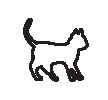
\includegraphics[width=150pt, height=150pt]{Chapters/chapter1/figures/cat.eps}}
%\caption[List of figure caption goes here]{Figure caption goes here. Figure caption goes here.}
%\end{figure}

%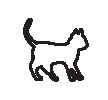
\includegraphics[width=\textwidth]{Chapters/chapter1/figures/cat.eps}
%\caption[Short figure caption]{Figure caption goes here.
%Figure caption goes here.
%Figure caption goes here.}
%\end{figure}

\section{Glossary}
\begin{Glossary}
\item[Adaptable] An adaptable process is designed to maintain effectiveness and
efficiency as requirements change. The process is deemed adaptable when there
is agreement among suppliers, owners, and customers that the process will meet
requirements throughout the strategic period.
\end{Glossary}

